\chapter{Theoretische Grundlagen}

Laut [ARVR] lässt sich eine Augmentierte Realität mit den nachfolgenden fünf Schritten realisieren:

\begin{enumerate}
    \item Videoaufnahme
    \item Tracking
    \item Registrierung
    \item Darstellung
    \item Ausgabe
\end{enumerate}

In diesem Kapitel werden die theoretischen Grundlagen der einzelnen Schritte erläutert. 

\section{Dreidimensionale Grafik}

Um Augmented Reality und verwandte Technologien zu verstehen, ist ein grundlegendes Verständnis der mathematischen und geometrischen Prinzipien erforderlich, die der Darstellung und Manipulation dreidimensionaler Objekte zugrunde liegen. Diese Prinzipien bilden die Basis für die Erzeugung und Interaktion mit virtuellen Szenen und Objekten. Im Folgenden werden die Konzepte zur Beschreibung, Transformation und Darstellung dreidimensionaler Objekte erläutert.

\subsection{Dreidimensionale Objekte}

In der Computergrafik werden dreidimensionale Objekte, auch als Modelle bezeichnet, durch geometrische und relationale Informationen beschrieben. Diese Objekte bestehen in der Regel aus Polygonen, die durch ihre Eckpunkte (Vertices) definiert sind. Ein Polygon ist eine geschlossene Fläche, die durch das Verbinden der Vertices mit geraden Linien entsteht. Jedem Vertex können zusätzliche Attribute wie Farbe, Texturkoordinaten oder Normalenvektoren zugewiesen werden.

Das einfachste Polygon ist ein Dreieck, das nur drei Eckpunkte benötigt. Dreiecke sind planar und konvex, was sie ideal für Berechnungen in der Computergrafik macht, wie beispielsweise bei der Beleuchtung oder Kollisionserkennung. Obwohl komplexere Polygone existieren, werden diese oft in Dreiecke zerlegt, da sie von Grafikpipelines effizienter verarbeitet werden können. Solche Modelle bestehen dann aus Dreiecksnetzen (Meshes), die als Arrays von Vertices und Indizes gespeichert werden.

\subsection{Welt- und lokale Koordinaten}

Virtuelle 3D-Szenen und Objekte werden in einem kartesischen Koordinatensystem beschrieben. Dieses Koordinatensystem wird üblicherweise als Weltkoordinatensystem bezeichnet, in dem die \(x\)-, \(y\)- und \(z\)-Achsen die drei Dimensionen repräsentieren. In einem rechtshändigen Koordinatensystem zeigt die \(x\)-Achse nach rechts, die \(y\)-Achse nach oben und die \(z\)-Achse nach vorne.

Jedes 3D-Objekt hat zusätzlich ein eigenes lokales Koordinatensystem. Die Vertices eines Objekts werden in diesem lokalen Koordinatensystem definiert. Um ein Objekt in der Szene zu platzieren, werden seine lokalen Koordinaten mithilfe von Transformationen in die Weltkoordinaten transformiert.

\subsection{Transformationen}

Transformationen werden verwendet, um Objekte in einer 3D-Szene zu verschieben, zu drehen oder zu skalieren. Diese Vorgänge werden durch Transformationsmatrizen beschrieben, die einheitlich auf alle Vertices eines Objekts angewendet werden. Solche Matrizen haben typischerweise die Größe \(4 \times 4\) und kombinieren Translation, Rotation und Skalierung.

\subsubsection{Translation (Verschiebung)}

Die Translation verschiebt ein Objekt entlang der \(x\)-, \(y\)- oder \(z\)-Achse. Die Transformationsmatrix für eine Translation ist wie folgt definiert:

\begin{equation}
\begin{bmatrix}
x' \\ y' \\ z' \\ 1
\end{bmatrix}
=
\begin{bmatrix}
1 & 0 & 0 & t_x \\
0 & 1 & 0 & t_y \\
0 & 0 & 1 & t_z \\
0 & 0 & 0 & 1
\end{bmatrix}
\begin{bmatrix}
x \\ y \\ z \\ 1
\end{bmatrix}
\end{equation}

Hierbei verschieben die Parameter \(t_x\), \(t_y\) und \(t_z\) das Objekt entlang der jeweiligen Achsen.

\subsubsection{Rotation (Drehung)}

Die Rotation eines Objekts erfolgt um eine der drei Achsen (\(x\), \(y\) oder \(z\)). Die Rotationsmatrizen sind für jede Achse wie folgt definiert:

\paragraph{Rotation um die \(x\)-Achse:}
\begin{equation}
\begin{bmatrix}
1 & 0 & 0 & 0 \\
0 & \cos(\alpha) & -\sin(\alpha) & 0 \\
0 & \sin(\alpha) & \cos(\alpha) & 0 \\
0 & 0 & 0 & 1
\end{bmatrix}
\end{equation}

\paragraph{Rotation um die \(y\)-Achse:}
\begin{equation}
\begin{bmatrix}
\cos(\alpha) & 0 & \sin(\alpha) & 0 \\
0 & 1 & 0 & 0 \\
-\sin(\alpha) & 0 & \cos(\alpha) & 0 \\
0 & 0 & 0 & 1
\end{bmatrix}
\end{equation}

\paragraph{Rotation um die \(z\)-Achse:}
\begin{equation}
\begin{bmatrix}
\cos(\alpha) & -\sin(\alpha) & 0 & 0 \\
\sin(\alpha) & \cos(\alpha) & 0 & 0 \\
0 & 0 & 1 & 0 \\
0 & 0 & 0 & 1
\end{bmatrix}
\end{equation}

Die Reihenfolge, in der Rotationen um verschiedene Achsen durchgeführt werden, ist entscheidend, da sie die endgültige Orientierung beeinflusst. Diese Reihenfolge wird durch Euler-Winkel beschrieben.

\subsubsection{Skalierung (Größenanpassung)}

Die Skalierung verändert die Größe eines Objekts proportional entlang der \(x\)-, \(y\)- und \(z\)-Achsen. Die Skalierungsmatrix ist wie folgt definiert:

\begin{equation}
\begin{bmatrix}
x' \\ y' \\ z' \\ 1
\end{bmatrix}
=
\begin{bmatrix}
s_x & 0 & 0 & 0 \\
0 & s_y & 0 & 0 \\
0 & 0 & s_z & 0 \\
0 & 0 & 0 & 1
\end{bmatrix}
\begin{bmatrix}
x \\ y \\ z \\ 1
\end{bmatrix}
\end{equation}

Hierbei sind \(s_x\), \(s_y\) und \(s_z\) die Skalierungsfaktoren entlang der jeweiligen Achsen.

\subsubsection{Anwendung der Transformationen}

Die lokalen Koordinaten eines Objekts können mithilfe einer Transformationsmatrix in Weltkoordinaten umgerechnet werden:

\begin{equation}
P_{world} = T_{object} \cdot P_{object}
\end{equation}

Hierbei ist \(T_{object}\) die Transformationsmatrix des Objekts, und \(P_{object}\) sind die lokalen Koordinaten. Das Ergebnis \(P_{world}\) beschreibt die Position des Objekts im Weltkoordinatensystem.

\section{Kalibrierung}

In Augmented-Reality-Anwendungen ist eine präzise Überlagerung digitaler Informationen auf die reale Welt essenziell, um ein realistisches und funktionales Benutzererlebnis zu schaffen. Die Kamerakalibrierung spielt hierbei eine entscheidende Rolle, da sie sicherstellt, dass virtuelle Objekte korrekt positioniert, skaliert und perspektivisch angepasst in die physische Umgebung integriert werden.

Die Kalibrierung umfasst die Bestimmung der \textbf{intrinsischen} und \textbf{extrinsischen} Parameter der Kamera:
\begin{itemize}
    \item \textbf{Intrinsische Parameter} beschreiben die optischen Eigenschaften der Kamera, wie Brennweiten, Verzerrungen und die Position des optischen Zentrums.
    \item \textbf{Extrinsische Parameter} legen die Position und Orientierung der Kamera im Raum fest, was für die korrekte Transformation zwischen Welt- und Bildkoordinaten erforderlich ist.
\end{itemize}

\begin{figure}
\centering
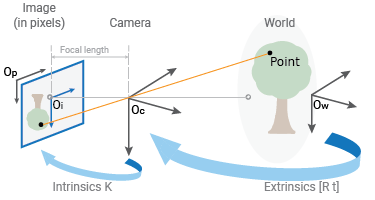
\includegraphics[ width=.5\textwidth ]{calibration-cameramodel-coords}
\caption{Modell für die Kamerakalibrierung\label{fig:Kalibrierung}}\par
\end{figure}

Mathematisch wird die Transformation durch die Gleichung \( x = PX \) beschrieben, wobei:
\begin{itemize}
    \item \( x \) die Bildkoordinaten in Pixeln sind,
    \item \( P \) die Projektionsmatrix ist und
    \item \( X \) die Weltkoordinaten eines Objekts darstellt.
\end{itemize}

Die Projektionsmatrix \( P \) setzt sich aus der intrinsischen Matrix \( K \) sowie der Rotationsmatrix \( R \) und dem Translationsvektor \( t \) zusammen:
\[
P = K[R|t]
\]

Die intrinsische Matrix \( K \) wird folgendermaßen definiert:
\[
K = 
\begin{bmatrix}
f_x & s & c_x \\
0 & f_y & c_y \\
0 & 0 & 1
\end{bmatrix}
\]
\begin{itemize}
    \item \( f_x \) und \( f_y \): Brennweiten der Kamera in Pixeln, bezogen auf die horizontalen und vertikalen Achsen.
    \item \( c_x \) und \( c_y \): Koordinaten des optischen Zentrums in Pixeln.
    \item \( s \): Skew-Faktor, der berücksichtigt, ob die Kameraachsen orthogonal sind.
\end{itemize}

Die Transformation von Weltkoordinaten in Bildkoordinaten wird schließlich durch die Matrix-Multiplikation berechnet:
\[
\begin{bmatrix}
x \\ y \\ 1
\end{bmatrix}
= 
\begin{bmatrix}
f_x & 0 & c_x \\
0 & f_y & c_y \\
0 & 0 & 1
\end{bmatrix}
\begin{bmatrix}
r_{11} & r_{12} & r_{13} & t_1 \\
r_{21} & r_{22} & r_{23} & t_2 \\
r_{31} & r_{32} & r_{33} & t_3
\end{bmatrix}
\begin{bmatrix}
X \\ Y \\ Z \\ 1
\end{bmatrix}
\]

Zur Kalibrierung werden in der Praxis oft visuelle Marker, wie Schachbrettmuster oder Würfel mit bekannten Geometrien, verwendet. Die Kamera erfasst diese Marker, und mithilfe einer Optimierung, z. B. durch Minimierung eines Fehlermaßes (Loss-Funktion), werden die Kameraparameter berechnet.

Um die Lens-Distortion zu korrigieren, werden oft Polynommodelle, wie das Brown-Conrady-Modell, verwendet. Dieses Modell beschreibt die radiale und tangentialen Verzerrungen der Linse und wird durch die Koeffizienten \( k_1, k_2, k_3 \) und \( p_1, p_2 \) definiert.

Moderne AR-Plattformen wie ARKit oder ARCore integrieren den Kalibrierungsprozess automatisch. ARKit speichert intrinsische Parameter in der Klasse \texttt{AVCameraCalibrationData} und berechnet die extrinsischen Parameter durch die Inertial Measurement Unit (IMU) des Geräts, welche Positions- und Orientierungsdaten liefert.

